% Chapter 3
\chapter{Event Reconstruction} % Main chapter title
\label{reco} 

\lhead{Chapter 3. \emph{Event Reconstruction}} % This is for the header on each page - perhaps a shortened title

%----------------------------------------------------------------------------------------

Event reconstruction is the process of computing quantities useful for physics analyses and constructing software objects called ``physics'' objects which are associated quantities that describe the kinematic properties of particles in an event.  It is a software operation which is fundamentally a data reduction procedure whose primary client is the data analysis.  Reconstruction can be divided in to 3 fundamental steps: local reconstruction that occurs within a single subdetector module, global reconstruction that occurs within a whole subdetector system, and the combination of the reconstructed objects to produce higher-level objects.  

Local reconstruction uses as input either real data acquired during runtime that was triggered on by the HLT and stored, or simulated data produced to represent the real data.  The data collected by the DAQ system is in the form of the digitized response of the various subsystems' modules to incident particles (charge avalanches, energy deposits in crystals, etc), so these input data objects are called ``digis'' - a reference to the fact that they are either digitized detector responses or simulations thereof.  The output of local reconstruction software is a reconstruction of the physical hit that occurred in the subdetector module.  Called a ``rechit'', these data objects are typically position measurements taken from times or clusters of strips or pixels in tracking-type subdetector systems (Muon and Tracker), and locations of energy cluster deposits in the calorimeters (ECAL and HCAL).  These rechits are used as input in the following reconstruction step.  

The global reconstruction step occurs separately for each subdetector, in which rechits from multiple subdetector modules are combined.  For instance, rechits from muons are used to produce reconstructed tracks representing candidate muon tracks and rechits in the tracker are used to produce reconstructed charged particle tracks.

Finally, the last step combines the reconstructed data objects from various individual subdetectors to produce the higher-level objects that are ultimately used in high-level triggering and/or for physics analyses.  As an example, a given track in the Tracker subsystem and a track in either the DT or CSC substem (Muon subdetectors) may be combined to form final muon candidates, and likewise electron candidates from the calorimeters are matched to tracks in the Tracker.  

The path that data from a muon takes through this reconstruction algorithm to eventually become a set of kinematics quantities identified as a ``Muon'' is depicted in Figure~\ref{figapp:CMSReco}.  In depth descriptions of the reconstruction of all physics objects follow in sections~\ref{trackreco} through~\ref{pflow}.

\begin{figure}[!Hh]
       \centering
       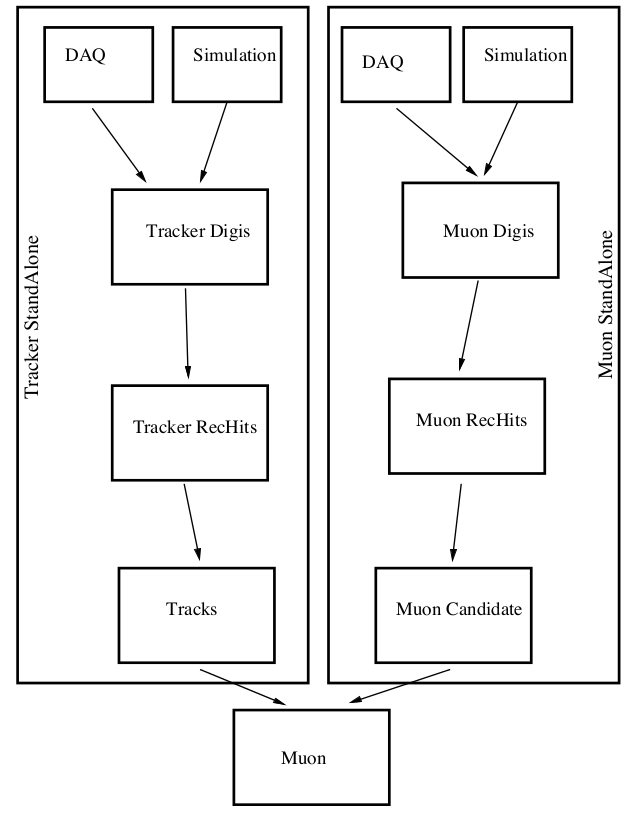
\includegraphics[scale=0.6]{Figures/CMSReco.png} \\
       \caption[A diagram of reconstruction of a muon in CMS.]{An example of a path that data from a muon takes through reconstruction, in the Tracker and Muon subsystems~\cite{CMStdr}.}
\label{figapp:CMSReco}
\end{figure}



\section{Track and Vertex Reconstruction}
\label{trackreco}

Tracks formed by charged particles in the tracking system are reconstructed via an iterative trajectory finding method called the Combinatorial Track Finder (CTF).  This method makes use of both pixel hits and strip hit in in local reconstruction, and pixel hits created via a fast algorithm are used for initial track seeding.  

For ``first-pass'' hit reconstruction, the transverse and longitudinal coordinates are determined via a simple computation.  For each coordinate the cluster is projected on to the respective axis, in the case of a single pixel the center of the pixel is taken, and if there are multiple pixels the hit position is determined using the relative charge of the two pixels at either end.  The position is then corrected for the Lorentz drift of the collected charge in the magnetic field.  These simple hit coordinates are used for track seeding, the first step of the global track reconstruction.  

Over the lifetime of the detector the radiation exposure can significantly impact a pixel module's collection of charge, and thus degrade the performance of the above standard hit reconstruction method.  The hit position can become biased by up to $50 \mu\text{m}$, so a template-based algorthim is used for the steps after track seeding in global track reconstruction~\cite{TrackReco}.  In this method the distribution of charge in the pixel module is compared to expected projected distributions in order to estimate hit positions.  These expected distrubions, called templates, are produced in a simulation called PIXELAV which can include descriptions of behavior of irradiated pixel sensors.  Thus, with updates over the course of the pixel tracker's lifetime, template-based algorithms can maintain a more realistic picture of sensor behavior and thus reduce position bias and improve resolution of the hit reconstruction.  

In the case of hit reconstruction in the strip detector, a seeding method is used.  Clusters are seeded by any channel that is saved offline that has a charge of at least three times the corresponding channel noise.  Neighboring strips are added to this seed if their charge it twice their strip noise, and a cluster overall is kept if the total charge is a factor of five larger than the total cluster noise.  The position of the hit for each cluster is then determined from the charge-weighted average of strip positions, corrected for Lorentz drift as well as for inefficient charge collection near the backplane of the sensitive strip volume.  These strip hits are used in the successive steps of global track reconstruction after seeding.


The global reconstruction of tracks takes the hits in the tracker subdetectors and estimates the momentum and positions of the charged particles responsible for those hits.  The momentum is computed from the bending of the trajectory of the particle in the magnetic field and thus the key role of the global reconstruction is to create these trajectories.  This is performed the software, mentioned above, called the CTF.  The CTF is an adaptation of the combinotorial Kalman filter~\cite{Kalman_Comb1,Kalman_Comb2,Kalman_Comb3} which is a basic Kalman filter~\cite{Kalman_Plain} that includes pattern recognition with track fitting in the same framework.   The CTF process is applied 6 times, iteratively, with the strategy of searching for the tracks that are easiest to find in the first iterations and the tracks that are hardest in the last iterations.  Thus the hits associated with tracks are removed in each iteration, reducing the combinatorial multiplicity in subsequent steps that search for more difficult track classes such as low-$p_T$ or displaced tracks.  Each iteration consists of four steps:

\begin{itemize}
\item{Seed generation begins by providing initial track candidates based on only two or three hits.  The seed contains the initial estimate of trajectory parameters with their uncertainties.}
\item{Finding the track is performed with a Kalman filter, extrapolating the seed trajectories along the expected path and searching for additional hits to be assigned to the track candidate.}
\item{Fitting the track is perfomed with a Kalman filter and smoother, to provide an improved estimate of the parameters of each trajectory.}
\item{Finally, track selection applies a set of quality criteria and discards tracks that fail it, as well as setting various quality flags on passing tracks}
\end{itemize}

The six successive iterations vary in how the inital seed is configured and the criteria applied in the final selection, with the same Kalman filter-based method applied to track finding and fitting.

The resolution of the reconstructed parameters of the tracks is studied using simulated events, using the differences between the generated values and the reconstructed values.  Figure~\ref{figapp:TrackRes} shows the $p_T$ resolution, as a percentage of $p_T$, for singly produced and isolated muons.



\begin{figure}[!Hh]
       \centering
       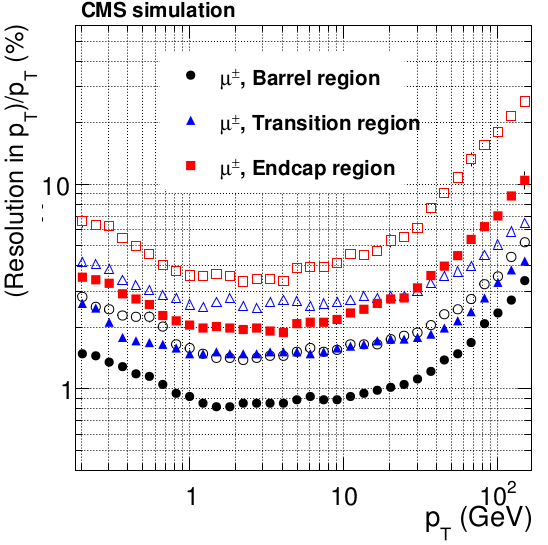
\includegraphics[scale=0.5]{Figures/TrackRes_pt.png} 
       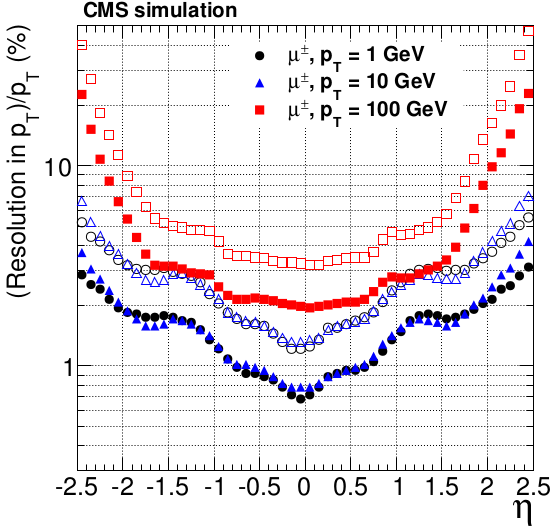
\includegraphics[scale=0.5]{Figures/TrackRes_eta.png} \\
       \caption[Transverse momentum resolution of tracks.]{Resolution of the track $p_T$, for singly produced and isolated muons with $p_T$=1,10, and 100 GeV.  The solid symbols represent the half-width for 68\% intervals, while open represents 90\%~\cite{TrackReco}.}
\label{figapp:TrackRes}
\end{figure}



Reconstruction of the primary vertex aims to measure the location and the associated uncertainty of all the proton-proton interaction vertices in each event, including the ``main'' event and any from pileup collisions, using the reconstructed tracks.  It is perfomed in three steps:


\begin{itemize}
\item{Track selection, in which tracks likely to have been produced ``promptly'' in the primary interaction region are chosen by imposing requirements on the maximum value of significance of the transverse impact parameter relative to the beam spot, the number of strip and pixel hits associated with the track, and the normalized $\chi^2$ from the trajectory fit~\cite{TrackReco}.}
\item{Clustering of tracks that appear to originate from the same interaction vertex, originally performed via simple ordering according to the z-coordinate of the point of closest approach of the tracks to the center of the beamspot and seperated in to different clusters when a given set of coordinates were seperated by more than 2 mm.  Proving a poor choice for high-pileup LHC conditions, this was later changed to a more complex association system called ``deterministic annealing''~\cite{} which included ``soft'' assignments, allowing tracks to be associated with more than one cluster.}
\item{Finally the candidate vertices are fitted to find its position and covariance matrices as well as parameters such as the number of degrees of freedom and weights of tracks used to indicate likelihood of success of the fit.  Each track is assigned a weight between 0 and 1 that reflects the likelihood it belongs to the vertex.}
\end{itemize}

The resolution of the reconstruced primary-vertex position is greatly dependent on the number of tracks used in the fit, as well as the $p_T$ of those tracks.  This dependence is shown in Figure~\ref{figapp:VertexRes}.


\begin{figure}[!Hh]
       \centering
       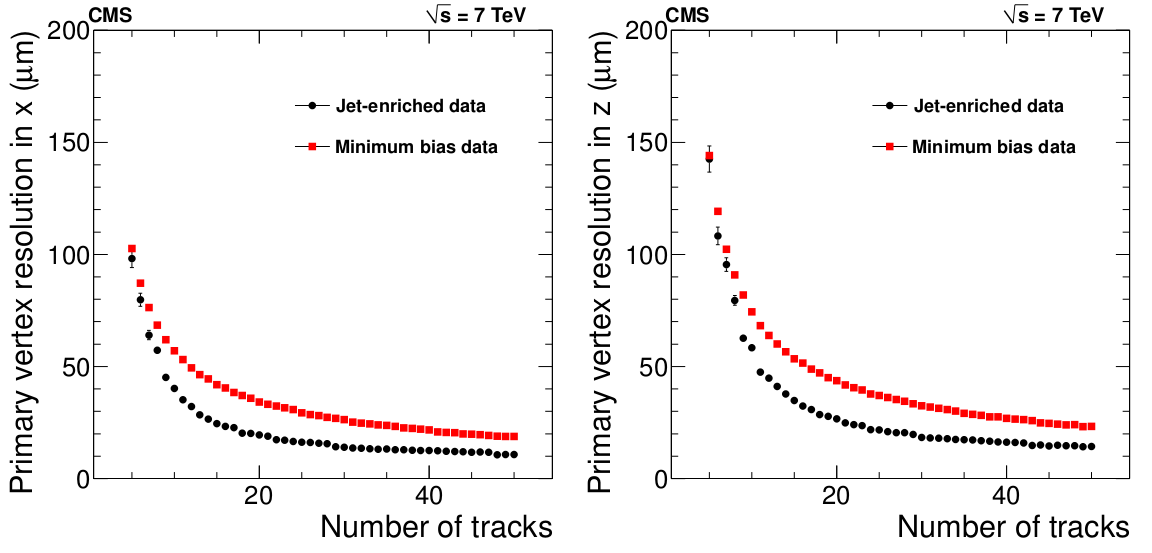
\includegraphics[scale=0.4]{Figures/VertexRes.png} \\
       \caption[Primary vertex resolution as a function of number of tracks.]{Primary vertex resolution as a function of the number of tracks in the vertex.  The jet-enchriched data contains tracks with a significantly higher $p_T$ values~\cite{TrackReco}.}
\label{figapp:VertexRes}
\end{figure}

\section{Muon Reconstruction}
\label{muonreco}

Other than neutrinos and other particles that only weakly interact and cannot be detected in any subdetector in CMS, muons are the only particles that pass through all the detectors inside the magnet solenoid and form tracks in the gas based muon system.  An example of a muon's path through CMS is shown in Figure~\ref{figapp:CMSSlice}.  The CSCs, DTs, and RPCs can form their own muon tracks as well as identify associated tracks from the tracker, and as a result muons are globally reconstructed in both the muon systems and in the tracker system.

\begin{figure}[!Hh]
       \centering
       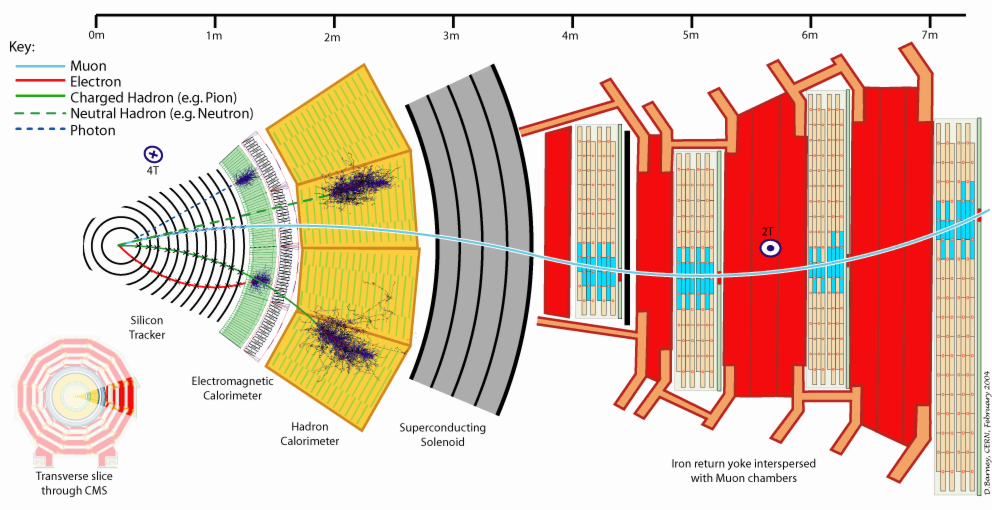
\includegraphics[scale=0.4]{Figures/CMS_Slice.png} \\
       \caption[A transverse slice of the CMS detector]{A slice of a the CMS detector, on the transverse plane, depicting various particles interacting with each specific subsystem.  A muon is shown in blue, traversing the tracker, calorimeters, and magnetic solenoid to leave a track in a muon system.  Its track is bent in two directions, in the inner 4 T field and the outer 2 T field.}
\label{figapp:CMSSlice}
\end{figure}

As with reconstruction in other subsystems, the muon systems begin their reconstruction with local reconstruction - building reconstructed hits either out of simulated data or actual collected data.  The main objects that the DTs use for this are hits in the volume of the drift cells, for which the drift times are converted to drift distances.  Separate $r-/phi$ and $r-z$ projections are combined in to 3-D ``rechits'' and a line segment is formed from aligned hits within the chamber.  The best segment candidate is chosen from any segments sharing hits, and in turn the hit information and segment fit is updated.  

A very similar method is used for the CSCs.  In each of the six layers of a CSC chamber the pulse height is measured to determine the probable hit position, and a 2-D hit is produced with local x and y positions based on the intersection of the locations on the strip and on the wire.  Then a segment is produced by connecting the first and last hits in a chamber, and including any hits within a clustering window along the line connecting those two hits.  This segment must pass a requirement on the resulting $\chi^2$/(number of degrees of freedom) of the fit of those hits that are included.  A minimum of three hits is required for each segment, although segments tend to include closer to the maximum possible 6 hits per segment (due to the 6 layers of the CSCs), as shown in Figure~\ref{figapp:SegmentsPerHit}.

\begin{figure}[!Hh]
       \centering
       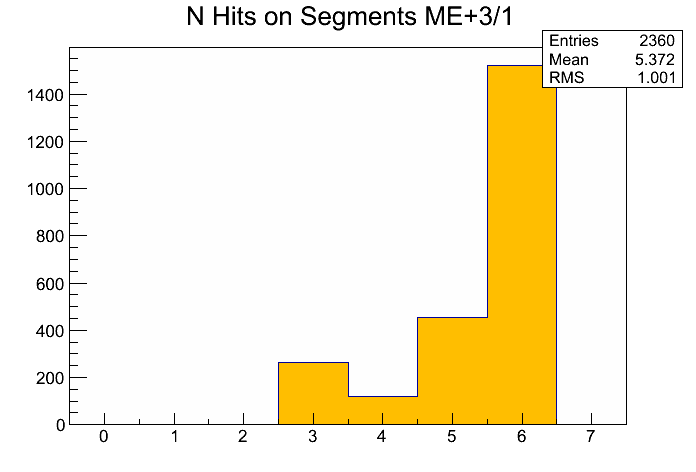
\includegraphics[width=0.45\textwidth]{Figures/Segments_hSnHits+31.png} 
       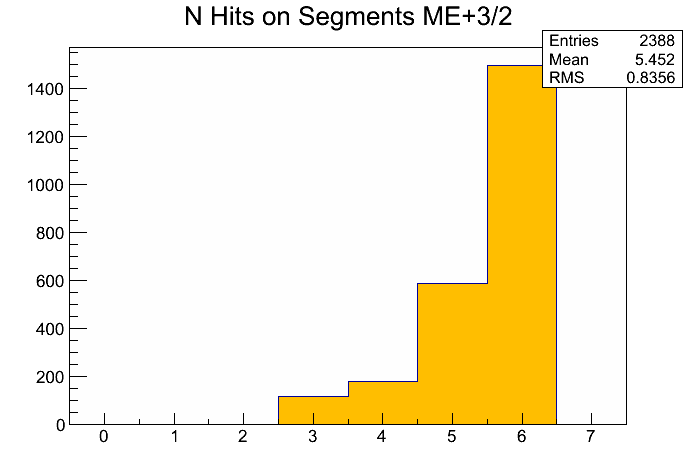
\includegraphics[width=0.45\textwidth]{Figures/Segments_hSnHits+32.png} \\
       \caption[Average hits per segment in a cathode strip chamber]{The average number of hits per segment for a given run in 2012.  The inside disk of the third station of the CSCs (left, ME+3/1) has slightly more ``showered'' muons than the outside disk of the same station (right, ME+3/2).}
\label{figapp:SegmentsPerHit}
\end{figure}

Finally, the RPCs are used in local reconstruction to obtain neighboring clusters with average positions that match the reconstructed hits in either the DTs or the CSCs.

Global reconstruction of muons begins with ``standalone'' reconstruction of tracks only in the muon chambers themselves, also called Level-2 reconstruction.  In standalone reconstruction, the track segments that are built during local reconstruction are used as seeds for muon trajectories.  The track segments from the innermost detectors are taken as state vectors (vectors containing their positions, direction, and momentum, along with covariance matrices) to start an inside-out Kalman fitting procedure~\cite{CMStdr,Kalman_Comb3}.  A predicted state vector is created at the next chamber by using the parameters of the initial state vector and propagating the trajectory outwards.  This projection takes the muon energy loss in the material, the effects of multiple scattering, and the nonuniformity of the magnetic field into account.  At that chamber, assuming that the actual track segment there passes a certain $\chi^2$ requirement, the predicted state is updated with the new information, adjusting parameters of the state vector for the next iteration.  Once the outermost chamber is reached, the ``Kalman Update'' step is complete, and an outside-in fit is performed in the exact same manner, in order to smooth the resulting trajectory.  Together with the ``Kalman Update'', this ``Kalman Smoothing'' step composes the entire Kalman Filter that is applied to the muon track segments.  In the DTs, since each hit is only 2-D, the entire segment is used for this procedure, but the CSC hits are 3-D so each hit is used individually.

Include from http://arxiv.org/pdf/1206.4071.pdf the global reco information, and the muon identification and muon sources information


\begin{figure}[!Hh]
       \centering
       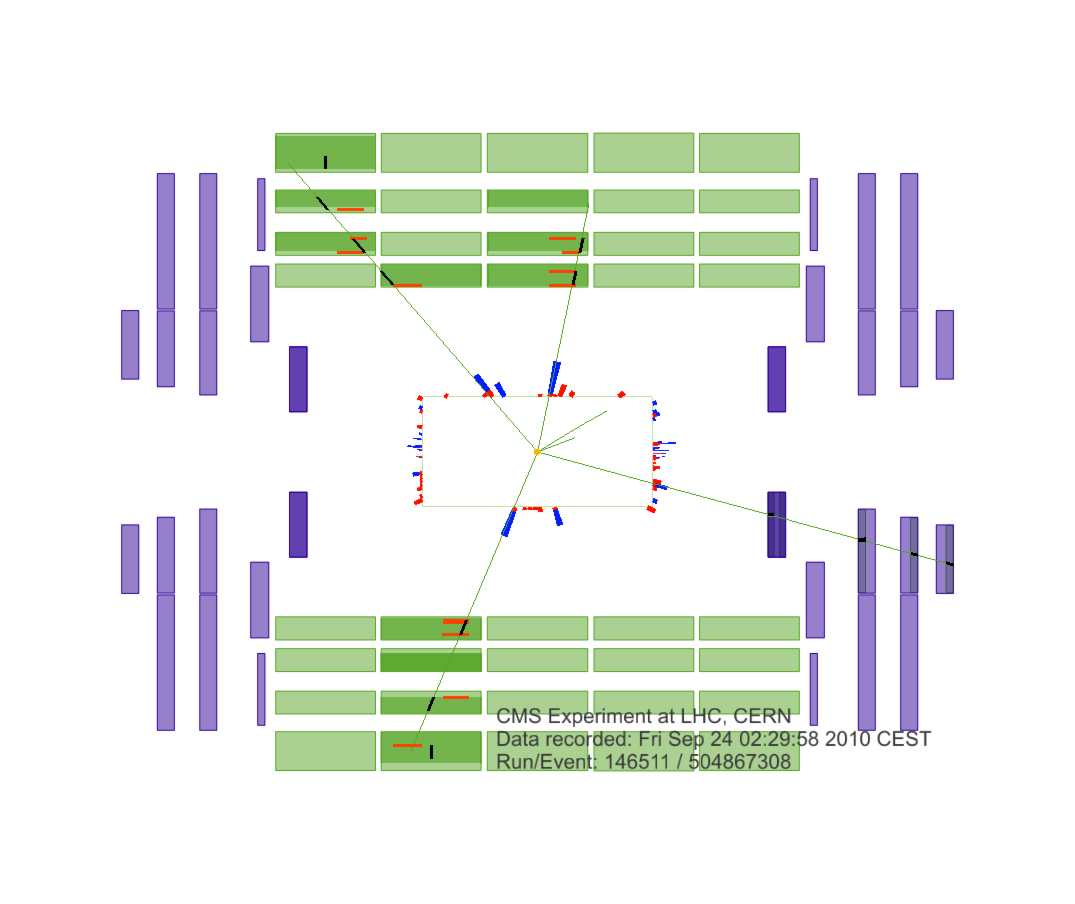
\includegraphics[scale=0.4]{Figures/pictures_r_z_4muon_event_diff_colors_1.png} \\
       \caption[An example of a four muon event in CMS]{A longitudinal view of a collision event in which four muons were reconstructed.  The thin green curves in the inner cylinder represent the tracks of charged particles which were reconstructed in the inner tracker with transverse momentum $p_T > 1\GeV/c$.  Those that extend to the muon system represent the tracks of muons that were reconstructed with both the inner tracker and teh muon system.  Three muons were detected by the DTs and RPCs, and the fourth by the CSCs.  The short black lines in the muon system show segments that were included in the moun track, and the horizontal red lines are depicted the positions of RPC hits.  The energy depositions are shown in red (for ECAL) and blue (for HCAL) on the outer edge of the inner cylinder.~\cite{Chatrchyan:2012xi}}
\label{figapp:ExampleEvent}
\end{figure}


--> muon seeds (from tracker/muon system)
--> L2/standalone reco, just in muon chambers  Kalman filter, propagator with average energy loss, etc, updates
--> L3/global reco with tracker info

--> Something about upgrade for ME0s - improvements of acceptance, etc  go back and put in references that may make sense to build to this point

\section{Electron Reconstruction}
\label{elereco}

\section{Particle flow and jets}
\label{pflow}



\section{Event simulation and detector response}
\label{simulation}
